\documentclass{article}

\usepackage{longtable}

\usepackage{indentfirst}

\usepackage[utf8]{inputenc}
\usepackage[T1]{fontenc}
\usepackage{fancyhdr}
\usepackage{geometry}
\usepackage{array}
\usepackage[usenames,dvipsnames,svgnames,table]{xcolor}
\usepackage{multirow}
\usepackage{morefloats}
\usepackage{float}
\usepackage{soul}
\usepackage{color}
\usepackage{seqsplit}
\usepackage{gensymb}
\usepackage{siunitx}
\usepackage{graphicx}
\usepackage{pdfpages}
\usepackage[framemethod=TikZ]{mdframed}
\setcounter{secnumdepth}{3}

\usepackage[procnames]{listings}
\usepackage{color}

\definecolor{keywords}{RGB}{255,0,90}
\definecolor{comments}{RGB}{0,0,113}
\definecolor{red}{RGB}{160,0,0}
\definecolor{green}{RGB}{0,150,0}

\lstset{language=Python,
        basicstyle=\ttfamily\small,
        keywordstyle=\color{keywords},
        commentstyle=\color{comments},
        stringstyle=\color{red},
        % showstringspaces=false,
        identifierstyle=\color{green},
        procnamekeys={def,class}}


\restylefloat{table}

\fontfamily{cmss}\selectfont

\geometry{top = 1in, bottom = 1in, left = 0.5in, right = 0.5in}

\setlength{\parindent}{4em}
\setlength{\parskip}{1em}
\renewcommand{\baselinestretch}{1.5}

\pagestyle{fancy}
\renewcommand{\footrulewidth}{1pt}
\lhead{Waggle Sensor Array}
\chead{Interface and Data Format Specification}
\rhead{Version 1.01}
\lfoot{Waggle Group}
\rfoot{park708@purdue.edu}

\setlength{\tabcolsep}{10pt}
\renewcommand{\arraystretch}{1.0}

%%%%%%%%%%%%%%%%%%%%%%%%%%%%%%%%%%%%%%%%%%%%%%%%%%%%%%%%%%%%%%%%%%%%%%%%%%%%

\begin{document}

\begin{titlepage}
  \vspace*{\stretch{1.0}}
  \begin{center}
        \Huge\textbf{\textsc{Interface and \\ Data Format Specification \\ for sensors \\
        \Large\textsc{(v2 sensor boards)}}}\\[0.5cm]
        \Large\textsc{Waggle Group \\ Waggle Sensor Array}\\[1cm]
        \large\textsc{November 2016, }
        \large\textsc{Version 1.01}\\
   \end{center}
   \vspace*{\stretch{2.5}}
\end{titlepage}

\tableofcontents
\newpage

\section{Physical Connections and Interfaces}

`v3 sensor boards' means a set of sensors which includs a v3.1 Airsense board, a v3.1 Lightsense board, a Chemsense board, and a alpha sensor.

\begin{figure}[h]
\begin{center}
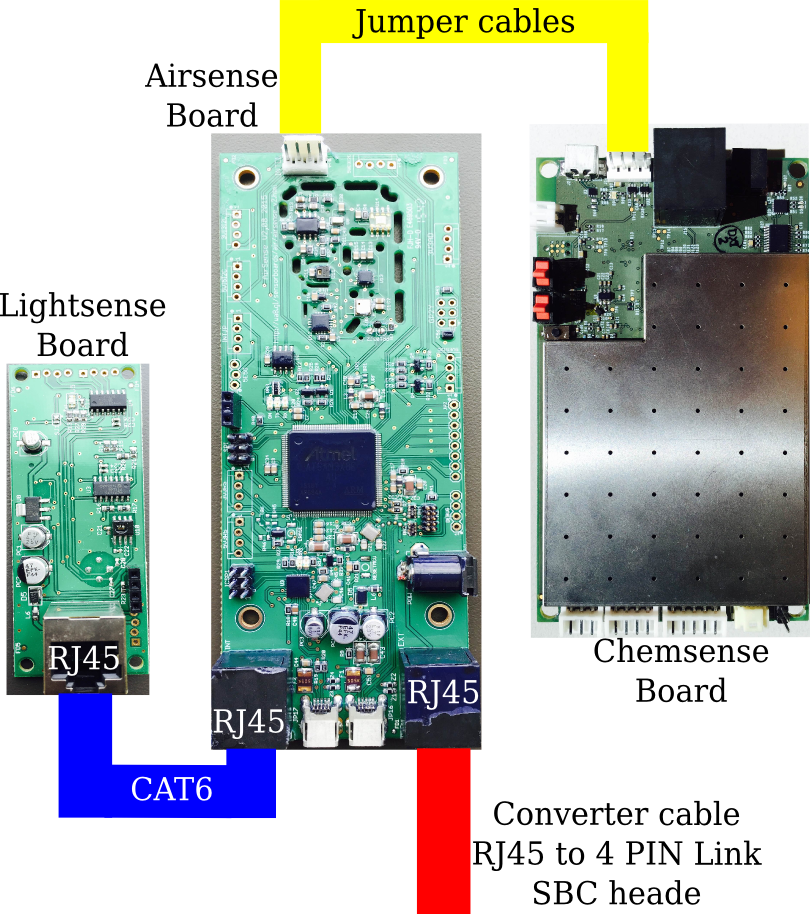
\includegraphics[width=4in]{g4353.png}
\caption{Connections between the sensor boards and the sensor}
\label{fig:physicalConnections}
\end{center}
\end{figure}

Physical connections between sensor boards and sensors are shown in the Figure \ref{fig:physicalConnections}. Airsense board is connected to lightsense board and chemsense board through CAT6 cable. Airsense and lightsense deliver data through I2C communication, and chemsense board delivers data through serial3 communication. All sensor data from airsense, lightsense, and chemsense board are delivered to nodecontroller thourgh USB connect attached on lightsense board. Alpha sensor will be conncted to Airsense board using SPI communication line. Then all the sensor data will be delivered through the USB connect on lighsense board.
\section{Data Transmission} \label{section:overall}

The data from the sensor boards is sent as a formatted unit of data -- a transmission
packet. A transmission packet is composed of several data sub-packets, each
of which carries information pertaining to the parameter listed in the sub-packet.
The data sub-packet, especially for additional sensors, rain gauge and soil moisture sensor, are described here.

\subsection{Data Sub-packets} \label{ssec:sub-pack}

The data segment of the transmission packet is further broken down into many
sub-packets. The sub-packet starts with a source identifier. One bit
validity field and seven bits ``length of the sub-packet'' field
are packed together as the next byte. The length field counts the number of
bytes following it which make up the sub-packet. The table below shows the organization
of a rain gauge sub-packet. 
\par
If the field is set to 1, it indicates a valid measurement/reading, 
and if the validity bit is set to 0 if the sensor represented in the sub-packet
is dead, disabled, unconnected, unresponsive or if data could not be collected
from the sensor in the time window. If the validity is 0, the particular invalid sub-packet is not packed into a transmission packet.

\subsubsection{Rain Gauge}
As shown in Table \ref{table:rain_subpacket}, sensor identifier of rain gauge is 0xFC, which is 252 in decimal, and if the data are valid, second byte will be 0x84, which means the sub-packet is valid and length of the sub-packet is 4 Bytes.


\begin{table}[H]
    \centering {
    \begin{tabular}{|c|c|c|c|}
        \hline
        \rowcolor{black!8}
        \textbf{Source ID} & \bf{1-bit Validity [0: invalid, 1: valid] | 7-bit Data Length} & \textbf{Data} \\
        \rowcolor{black!8}
        (1 Byte) & (1 Byte) & (2 Bytes) \\
        \hline
        0xFC & 0x84 (valid) & count of pendant event\\ 
        \hline
    \end{tabular}
    }
    \caption{Sub-packet for rain gauge}
    \label{table:rain_subpacket}
\end{table}


\subsubsection{Soil Moisture Sensor}
As shown in Table \ref{table:soil_subpacket}, sensor identifier of soil sensor is 0xFB, which is 251 in decimal,
and if the data are valid, second byte will be 0x84, which means the sub-packet is valid and length of the sub-packet is
6 Bytes.


\begin{table}[H]
    \centering {
    \begin{tabular}{|c|c|c|c|c|}
        \hline
        \rowcolor{black!8}
        \textbf{Source ID} & \bf{1-bit Validity | 7-bit Data Length} & \textbf{Data} \\
        \rowcolor{black!8}
        (1 Byte) & [0: invalid, 1: valid]  (1 Byte) & (6 Bytes) \\
        \hline
        \multirow{3}{*}{0xFB} & \multirow{3}{*}{0x86 (valid)} & Dielectric permittivity in Format 6 (2 Bytes) \\ \cline{3-3}
        & & Electric Conductivity in Format 6 (2 Bytes) \\ \cline{3-3}
        & & Temperature in Format 6 (2 Bytes) \\ \hline
    \end{tabular}
    }
    \caption{Sub-packet for rain gauge}
    \label{table:soil_subpacket}
\end{table}


\subsection{Data Formats}

The data sent in each sub-packet is encoded in one or more formats. Currently we define eight formats for various types of data including integers, bytes, and floating point numbers. 
Rain gauge data encoded as format 1, which is integers in range 0 to 65535, as shown in Table \ref{table:rain_format}.
Therefore the data of the rain gauge is an integer, and it means the count of pendant event inside the rain gauge. One event of the pendant means 0.01 in. (0.254 mm) of precipitation.
Soil sensor data is encoded as format 6, which is integers in range $-$127.99 to 127.99, as shown in Table \ref{table:rain_format}.
Therefore the data of the soil sensor are float point dielectric, conductivity, and temperature.
\\


\begin{table}[H]
    \centering {
    \begin{tabular}{|c|c|c|c|}
        \hline
        \rowcolor{black!8}
        \textbf{Format} & \textbf{Number of Bytes Used} & \textbf{Value Represented} & \textbf{Value Range} \\
        \hline
        1 & 2 & unsigned int\_16 input & 0 -- 65535 \\ %& MSByte LSByte\\
        6 & 2 & float input & [$-$127.99, 127.99] \\
        \hline
    \end{tabular}
    }
    \caption{Data format for rain gauge}
    \label{table:rain_format}
\end{table}

\clearpage
% \section{Data Sub-Packet} \label{section:dataSub}
%
% The data sub-packet consists of 32 "chunks" (30 sensors and 2 MAC addresses).  Each "chunk" follows one of seven formats.\\

%%%%%%%%%%%%%%%%%%%%
\newpage
\section{Data Formats}

The data sent in each sub-packet is encoded in one or more formats. Currently
we define eight formats for various types of data including integers, bytes,
and floating point numbers. The numerical range of these representations is
restricted to within the bounds of values that we expect from the various sensors
and other sources. Thus the encoding schemes are specifically designed to
effectively and efficiently encode the values expected in the sensor streams.
The eight formats, and the encoding schemes are listed below.

\begin{table}[H]
    \centering
    {\rowcolors{2}{black!8}{black!2}
    \begin{tabular}{|c|c|c|c|}
        \hline
        \textbf{Format} & \textbf{Number of Bytes Used} & \textbf{Value Represented} & \textbf{Value Range} \\
%          & \textbf{Encoding}
        \hline
        \hline
        1 & 2 & unsigned int\_16 input & 0 -- 65535 \\ %& MSByte LSByte\\
        2 & 2 & int\_16 input & $\pm$\{0 -- 32767\} \\%& [1Sign|7-MSBits] LSByte \\
        3 & 6 & byte input[6] & 0x00 -- 0xffffffffffff \\%& MSByte1 MSByte2 MSByte3 MSByte4 MSByte5 LSByte \\
        4 & 3 & unsigned long\_24 input & 0 -- 16777215 \\%& MSByte1 MSByte2 LSByte \\
        5 & 3 & long\_24 input & $\pm$\{0 -- 8388607\} \\%& [1Sign|7-MSBits] MSByte2 LByte \\
        6 & 2 & float input & $\pm$\{0 -- 127.99\} \\%& [1Sign|7Bits\_Int] [0|7Bits\_Frac]\\
        7 & 4 & byte input[4] & 0x00 -- 0xffffffff \\%& MSByte1 MSByte2 LSByte2 LSByte\\
        8 & 2 & float input & $\pm$\{0 -- 31.999\} \\%& [1Sign|5Bits\_Int|2MSBits\_Frac]  8LSBits\_Frac\\
        \hline
    \end{tabular}
    }
    \caption{Data formats}
    \label{table:overall}
\end{table}

%%%%%%%%%%%%%%%%%%%%

\subsection{Format 1}

This 2 byte format is used to transmit an integer between 0 and 65535. The
number is split and serialized as follows --\\

\begin{table}[H]
\centering
\begin{tabular}{|c|c|}
\hline
% column1a & column2a \\
\noalign{\hrule height 2pt}
\multicolumn{1}{!{\vrule width 2pt}c!{\vrule width 1pt}}{8 Most Significant Bits} &
  \multicolumn{1}{!{\vrule width 1pt}c!{\vrule width 2pt}}{8 Least Significant Bits} \\
\noalign{\hrule height 2pt}
Byte[0] & Byte[1] \\
\hline
\end{tabular}
\end{table}


\subsection{Format 2}
This 2 byte format is used to transmit an integer between -32767 and 32767. The
number is split and serialized as follows --\\

\begin{table}[H]
\centering
\begin{tabular}{|c|c|}
\hline
% column1a & column2a \\
\noalign{\hrule height 2pt}
\multicolumn{1}{!{\vrule width 2pt}c!{\vrule width 1pt}}{Sign Bit | 7 Most Significant Bits} &
\multicolumn{1}{!{\vrule width 1pt}c!{\vrule width 2pt}}{8 Least Significant Bits} \\
\noalign{\hrule height 2pt}
Byte[0] & Byte[1] \\
\hline
\end{tabular}
\end{table}

The Sign Bit which is the most significant bit in Byte 0 is set as follows ---

\begin{table}[H]
\centering
\begin{tabular}{|c|c|}
\hline
Positive Integer & 0 \\ 
\hline
Negative Integer & 1 \\
\hline
\end{tabular}
\end{table}



\subsection{Format 3}

This 6 byte format is used to transmit an array of 6 bytes. The array is serialized as follows --\\

\begin{table}[H]
\centering
\begin{tabular}{|c|c|c|c|c|c|}
\hline
% column1a & column2a \\
\noalign{\hrule height 2pt}
\multicolumn{1}{!{\vrule width 2pt}c!{\vrule width 1pt}}{Array[0]} &
\multicolumn{1}{!{\vrule width 2pt}c!{\vrule width 1pt}}{Array[1]} &
\multicolumn{1}{!{\vrule width 2pt}c!{\vrule width 1pt}}{Array[2]} &
\multicolumn{1}{!{\vrule width 2pt}c!{\vrule width 1pt}}{Array[3]} &
\multicolumn{1}{!{\vrule width 2pt}c!{\vrule width 1pt}}{Array[4]} &
\multicolumn{1}{!{\vrule width 1pt}c!{\vrule width 2pt}}{Array[5]} \\
\noalign{\hrule height 2pt}
1st Byte & 2nd Byte & 3rd Byte & 4th Byte & 5th Byte & 6th Byte \\
\hline
\end{tabular}
\end{table}

\subsection{Format 4}

This 3 byte format is used to transmit an integer between 0 and 16777215. The
number is split and serialized as follows --\\

\begin{table}[H]
\centering
\begin{tabular}{|c|c|c|}
\hline
% column1a & column2a \\
\noalign{\hrule height 2pt}
\multicolumn{1}{!{\vrule width 2pt}c!{\vrule width 1pt}}{8 Most Significant Bits} &
\multicolumn{1}{!{\vrule width 2pt}c!{\vrule width 1pt}}{Bits 15 -- 8 } &
  \multicolumn{1}{!{\vrule width 1pt}c!{\vrule width 2pt}}{8 Least Significant Bits} \\
\noalign{\hrule height 2pt}
Byte 0 & Byte 1 & Byte 2\\
\hline
\end{tabular}
\end{table}

\subsection{Format 5}

This 3 byte format is used to transmit an integer between -8388607 and 8388607. The
number is split and serialized as follows --\\

\begin{table}[H]
\centering
\begin{tabular}{|c|c|c|}
\hline
% column1a & column2a \\
\noalign{\hrule height 2pt}
\multicolumn{1}{!{\vrule width 2pt}c!{\vrule width 1pt}}{Sign Bit | 7 Most Significant Bits} &
\multicolumn{1}{!{\vrule width 2pt}c!{\vrule width 1pt}}{Bits 15 -- 8 } &
  \multicolumn{1}{!{\vrule width 1pt}c!{\vrule width 2pt}}{8 Least Significant Bits} \\
\noalign{\hrule height 2pt}
Byte 0 & Byte 1 & Byte 2\\
\hline
\end{tabular}
\end{table}

The Sign Bit which is the most significant bit in Byte 0 is set as follows ---

\begin{table}[H]
\centering
\begin{tabular}{|c|c|}
\hline
Positive Integer & 0 \\
\hline
Negative Integer & 1 \\
\hline
\end{tabular}
\end{table}



\subsection{Format 6}

This 2 byte format is used to transmit a floating point number between
-127.99 and 127.99. Only 2 fractional places are allowed in this format and
the number is serialized as follows --\\

\begin{table}[H]
\centering
\begin{tabular}{|c|c|c|c|c|c|}
\hline
% column1a & column2a \\
\noalign{\hrule height 2pt}
\multicolumn{1}{!{\vrule width 2pt}c!{\vrule width 1pt}}{Sign Bit| 7 bit representation of Integer part} &
\multicolumn{1}{!{\vrule width 2pt}c!{\vrule width 1pt}}{ 0 | 7 bit representation of the Fractional part} \\
\noalign{\hrule height 2pt}
Byte 0 & Byte 1\\
\hline
\end{tabular}
\end{table}

As shown above, the leading bit of the Byte 1 is always set to 0, and
the Sign Bit which is the most significant bit of Byte 0 is set as follows ---

\begin{table}[H]
\centering
\begin{tabular}{|c|c|}
\hline
Positive Number & 0 \\
\hline
Negative Number & 1 \\
\hline
\end{tabular}
\end{table}


\subsection{Format 7}

This 4 byte format is used to transmit an array of 4 bytes. The array is serialized as follows --\\

\begin{table}[H]
\centering
\begin{tabular}{|c|c|c|c|c|c|}
\hline
% column1a & column2a \\
\noalign{\hrule height 2pt}
\multicolumn{1}{!{\vrule width 2pt}c!{\vrule width 1pt}}{Array[0]} &
\multicolumn{1}{!{\vrule width 2pt}c!{\vrule width 1pt}}{Array[1]} &
\multicolumn{1}{!{\vrule width 2pt}c!{\vrule width 1pt}}{Array[2]} &
\multicolumn{1}{!{\vrule width 2pt}c!{\vrule width 1pt}}{Array[3]}\\
\noalign{\hrule height 2pt}
Byte 0 & Byte 1 & Byte 2 & Byte 3 \\
\hline
\end{tabular}
\end{table}


\subsection{Format 8}

This 2 byte format is used to transmit a floating point number between
-31.999 and 31.99. Only 3 fractional places are allowed in this format and
the number is serialized as follows --\\

\begin{table}[H]
\centering
\begin{tabular}{|c|c|c|c|c|c|}
\hline
% column1a & column2a \\
\noalign{\hrule height 2pt}
\multicolumn{1}{!{\vrule width 2pt}c!{\vrule width 1pt}}{Sign Bit| 5 bit representation of Integer | 2 most significant bits of fraction} &
\multicolumn{1}{!{\vrule width 2pt}c!{\vrule width 1pt}}{ 8 least significant bits of the fraction} \\
\noalign{\hrule height 2pt}
Byte 0 & Byte 1\\
\hline
\end{tabular}
\end{table}

As shown above, the format uses 5 bits for representing the integer part and 10 bits to represent the
fractional part. The Sign Bit which is the most significant bit of Byte 0 is set as follows ---

\begin{table}[H]
\centering
\begin{tabular}{|c|c|}
\hline
Positive Number & 0 \\
\hline
Negative Number & 1 \\
\hline
\end{tabular}
\end{table}


\newpage
\section{Sub-packets}

As shortly explained in document section \ref{ssec:sub-pack}, data sub-packets are generated depending on its designated data format and length when data reading from each sensor if valid. The first byte of the sub-packet is sensor ID for each parameter, and the second byte means validity of the packet and length of the sensor data as shown in Table \ref{table:packsegments}. Detail of sub-packet and sensor data will be explined in this section.


\subsection{Parameters}

The sensor boards output a set of parameters which are identified by a unique ID. Each parameter
has a set of values associated with it which are encoded in an appropriate data format. The table
below lists the various parameters produced by the sensor boards, the unique source ID used to identify them, the values produced by them and the format in which the value is encoded.
\par
Each parameter and its values are composed into a sub-packet based on
the format described in document section \ref{ssec:sub-pack}.
In the case of parameters with 2 or more values, the encoded values are
arranged in the sub-packets sequentially. 


\begin{center}
\begin{longtable}{|l|c|>{\centering}p{0.3\textwidth}|c|}
\caption{Data sub-packet structure (each row is a "chunk")} \label{tab:dataChunk} \\

\hline \rowcolor{black!8} \multicolumn{1}{|c|}{\textbf{Parameter}} & \multicolumn{1}{c|}{\textbf{Source ID}} & \multicolumn{1}{c|}{\textbf{Values}} & \multicolumn{1}{c|}{\textbf{Formats}} \\ \hline
\endfirsthead

\multicolumn{4}{c}%
{{\bfseries \tablename \thetable{} -- continued from previous page}} \\
\hline \rowcolor{black!8} \multicolumn{1}{|c|}{\textbf{Parameter}} & \multicolumn{1}{c|}{\textbf{Source ID}} & \multicolumn{1}{c|}{\textbf{Values}} & \multicolumn{1}{c|}{\textbf{Formats}} \\ \hline 
\endhead

% \rowcolor{black!8} \multicolumn{4}{|r|}{{Continued on next page}} \\ \hline
\endfoot

\hline
\endlastfoot

        \multirow{3}{*}{Firmware version} & \multirow{3}{*}{0xFD} & Firmware version (HW/SW) & \multirow{3}{*}{Bit mask} \\ \cline{3-3}
        & & Build time & \\ \cline {3-3} 
        & & Build git & \\ \hline

    \rowcolor{black!5} \multicolumn{4}{|c|}{{Airsense board}} \\ \hline
        Airsense/Lightsense MAC address & 0x00 & MAC Address & Format 3 \\ \hline
        TMP112 & 0x01 & Temperature & Format 6\\ \hline
        \multirow{2}{*}{HTU21D} & \multirow{2}{*}{0x02} & Temperature & \multirow{2}{*}{Format 6}\\ \cline{3-3}
        & & relative humidity & \\ \hline
        \multirow{2}{*}{BMP180} & \multirow{2}{*}{0x04} & Temperature & Format 6\\ \cline{3-4}
        & & Pressure & Format 4 \\ \hline
        PR103J2 & 0x05 & Temperature & Format 1\\ \hline
        TSL250RD & 0x06 & Visible Light & Format 1\\ \hline
        \multirow{4}{*}{MMA8452Q} & \multirow{4}{*}{0x07} & Acceleration in X & \multirow{4}{*}{Format 6}\\ \cline{3-3}
        & & Acceleration in Y & \\ \cline{3-3}
        & & Acceleration in Z & \\ \cline{3-3}
        & & Vibration & \\ \hline
        SPV1840LR5H-B & 0x08 & RMS Sound Level & Format 1\\ \hline
        TSYS01 & 0x09 & Temperature & Format 6\\ \hline
        
    \rowcolor{black!8} \multicolumn{4}{|c|}{{Lightsense board}} \\ \hline
        \multirow{3}{*}{HMC5883L} & \multirow{3}{*}{0x0A} & Magnetic Field in Z & \multirow{3}{*}{Format 8}\\ \cline{3-3}
        & & Magnetic Field in Y & \\ \cline{3-3}
        & & Magnetic Field in Z & \\ \hline
        \multirow{2}{*}{HIH6130} & \multirow{2}{*}{0x0B} & Temperature & \multirow{2}{*}{Format 6}\\ \cline{3-3}
        & & relative humidity & \\ \hline
        APDS-9006-020 & 0x0C & Ambient light intensity & Format 1\\ \hline
        TSL260RD & 0x0D & IR intensity & Format 1\\ \hline
        TSL250RD & 0x0E & Visible light intensity & Format 1\\ \hline
        MLX75305 & 0x0F & Light & Format 1\\ \hline 
        ML8511 & 0x10 & UV intensity & Format 1\\ \hline
        TMP421 & 0x13 & Temperature & Format 6\\ \hline
        SPV1840LR5H-B & 0x14 & RMS Sound Level & Format 1\\ \hline

    \rowcolor{black!8} \multicolumn{4}{|c|}{{Chemsense board}} \\ \hline
        Total reducing gases & 0x15 & \multirow{7}{*}{Raw Concentration} & \multirow{7}{*}{Format 5}\\ \cline{1-2}
        Nitrogen dioxide & 0x17 & & \\ \cline{1-2}
        Ozone & 0x18 & & \\ \cline{1-2}
        Hydrogen sulphide & 0x19 & &\\ \cline{1-2}
        Total oxidizing gases & 0x1A & &\\ \cline{1-2}
        Carbon monoxide & 0x1B & &\\ \cline{1-2}
        Sulfur dioxide & 0x1C & &\\ \hline
        \multirow{2}{*}{SHT25} & \multirow{2}{*}{0x1D} & Temperature & \multirow{2}{*}{Format 2}\\ \cline{3-3}
        & & relative humidity & \\ \hline
        \multirow{2}{*}{LPS25H} & \multirow{2}{*}{0x1E} & Temperature & Format 2\\ \cline{3-4}
        & & Pressure & Format 4\\ \hline
        \multirow{3}{*}{Si1145} & \multirow{3}{*}{0x1F} & UV intensity & \multirow{3}{*}{Format 1} \\ \cline{3-3}
        & & Visible light intensity & \\ \cline{3-3}
        & & IR intensity & \\ \hline
        Chemsense MAC address & 0x20 & MAC Address & Format 3\\ \hline
        CO ADC temp & 0x21 & \multirow{2}{*}{ADC temperature} &  \multirow{2}{*}{Format 2}\\ \cline{1-2}
        IAQ IRR ADC temp & 0x22 & &\\ \hline
        O3 NO2 ADC temp & 0x23 & \multirow{3}{*}{ADC temperature} &  \multirow{3}{*}{Format 2} \\ \cline{1-2}
        SO2 H2S ADC temp & 0x24 & & \\ \cline{1-2}
        CO LMP temp & 0x25 & &\\ \hline
        \multirow{4}{*}{Accelerometer} & \multirow{4}{*}{0x26} & Acceleration in X & \multirow{3}{*}{Format 2} \\ \cline{3-3}
        & & Acceleration in Y & \\ \cline{3-3}
        & & Acceleration in Z & \\ \cline{3-4}
        & & Vibration & Format 4\\ \hline
        \multirow{4}{*}{Gyro} & \multirow{4}{*}{0x27} & Orientation in X & \multirow{3}{*}{Format 2} \\ \cline{3-3}
        & & Orientation in Y & \\ \cline{3-3}
        & & Orientation in Z & \\ \cline {3-4}
        & & Orientation Index & Format 4\\ \hline

     \rowcolor{black!8} \multicolumn{4}{|c|}{{Alpha Sensor}} \\ \hline
        \multirow{9}{*}{Histogram} & \multirow{9}{*}{0x28} & Bin count & \multirow{20}{*}{Raw reading} \\ \cline{3-3}
        & & Average Time &\\ \cline{3-3}
        & & Sample flow rate &\\ \cline{3-3}
        & & Temp/Pressure(alther) &\\ \cline{3-3}
        & & Sampling period &\\ \cline{3-3}
        & & Sum of the counts &\\ \cline{3-3}
        & & PM 1 &\\ \cline{3-3}
        & & PM 2.5 &\\ \cline{3-3}
        & & PM 10 &\\ \cline{1-3}
        Firmware & 0x29 & Firmware version & \\ \cline{1-3}
        \multirow{2}{*}{Configuration A} & \multirow{2}{*}{0x30} & Bin Boundaries &\\ \cline{3-3}
        & & Bin Particle Volumes A &\\ \cline{1-3}
        \multirow{2}{*}{Configuration B} & \multirow{2}{*}{0x31} & Bin Particle Volumes B &\\ \cline{3-3}
        & & Bin Particle Densities A &\\ \cline{1-3}
        \multirow{2}{*}{Configuration C} & \multirow{2}{*}{0x32} & Bin Particle Densities B &\\ \cline{3-3}
        & & Bin Sample Volume Weightings A &\\ \cline{1-3}
        \multirow{6}{*}{Configuration D} & \multirow{6}{*}{0x33} & Bin Sample Volume Weightings B &\\ \cline{3-3}
        & & Gain Scaling Coefficient & \\ \cline{3-3}
        & & Sample Flow Rate & \\ \cline{3-3}
        & & Laser DAC and Fan DAC & \\ \cline{3-3}
        & & Conversion factor & \\ \cline{3-3}
        & & Space Bytes & \\ 

\end{longtable}
\end{center}


\subsection{Data packets}
The context of each parameter, its utility and the arrangement of its values is described below. In all
the tables below, the validity bit is set to 1, which means the data is valid. The parameter descriptions
below are aggregated based on the sensor-board they are situated on -
Metsense, Lightsense and Chemsense.

\subsubsection{Firmware Version}
This is a 8 bytes version information that identifies hardware version, software version, and build information of the waggle node.
The build time and the build git are included to varify the effectiveness of the software.
Firmware version is bit masked and encoded through format 1, and build git is encoded through format 1.

\begin{table}[h!]
    \centering
    \caption{Sub-packet of Firmware version}
    \begin{tabular}{|c|c|c|c|c|}
        \hline
        \rowcolor{black!8}
        \textbf{0xFD} & \textbf{0x88} & \textbf{Firmware version in Format 1} & \textbf{Build time} & \textbf{Build git in Format 1} \\ \hline
        Byte[0] & Byte[1] & Bytes[2 -- 3] & Bytes[4 -- 7] & Bytes[8 -- 9]\\ \hline
    \end{tabular}
\end{table}


\newcolumntype{a}{>{\columncolor{black!8}}c}
\begin{table}[h!]
    \centering
    \caption{Firmware version}
    \begin{tabular}{|a|c|}
        \hline
        \textbf{3 bit major HW ver. | 3 bit minor HW ver. | 2 bit major SW ver.} & Byte[2] \\ \hline
        \textbf{2 bit major SW ver. | minor SW ver. $\times$ 10 + sub SW ver.} & Byte[3]\\ \hline
    \end{tabular}
\end{table}

\newpage
\section{Sensor Data Units}\label{section:parameterUnits}
\subsection { Raw and Processed} 


The sensor boards output a set of values which have various units for the data.
The table below lists the various units of sensor values.
`Raw Units' in the table means the unit of the packtized data, which is you can get directly from the packet, and `Processed Units' means the unit which can be used after data conversion through designated equations.
The equations will be provided comming subsections.


\begin{center}
\begin{longtable}{|l|c|c|c|}
\caption{Sensor units both in raw and processed format}
\label{table:parameterUnits} \\

\hline \rowcolor{black!8} \multicolumn{1}{|l|}{\textbf{Sensor/Parameter}} & \multicolumn{1}{c|}{\textbf{Raw Units}} & \multicolumn{1}{c|}{\textbf{Processed Units}} & \multicolumn{1}{c|}{\textbf{Comments}} \\ \hline
\endfirsthead

\multicolumn{4}{c}%
{{\bfseries \tablename\ \thetable{} -- continued from previous page}} \\

\hline \rowcolor{black!8} \multicolumn{1}{|l|}{\textbf{Sensor/Parameter}} & \multicolumn{1}{c|}{\textbf{Raw Units}} & \multicolumn{1}{c|}{\textbf{Processed Units}} & \multicolumn{1}{c|}{\textbf{Comments}} \\ \hline
\endhead

\rowcolor{black!8} \multicolumn{4}{|r|}{{Continued on next page}} \\ \hline
\endfoot

\hline
\endlastfoot
 
    Firmware version & No Units & & *See appendix A \\ \hline

  \rowcolor{black!5} \multicolumn{4}{|c|}{{Airsense board}} \\ \hline
    Air/Lightsense MAC & No Units & No Units & \\  \hline
    TMP112 & \degree C & \degree C & \\ \hline
    HTU21D & \degree C, \%RH & \degree C, \%RH & \\ \hline
    BMP180 & \degree C, Pa & \degree C, Pa & \\ \hline
    PR103J2 & integer & \degree C & \\ \hline
    TSL250RD & integer & $\mu$w/m$^2$ & \\  \hline
    MMA8452Q & g, g, g, g & g, g, g, g & \\ \hline
    SPV1840LR5H-B & integer & & \\ \hline
    TSYS01 & \degree C & \degree C & \\ \hline
    
  \rowcolor{black!5} \multicolumn{4}{|c|}{{Lightsense board}} \\ \hline
    HMC5883L & G, G, G & G, G, G & \\ \hline
    HIH6130 & \degree C, \%RH & \degree C, \%RH & \\ \hline
    APDS-9006-020 & integer & lux & \\  \hline
    TSL260RD & integer & $\mu$w/m$^2$ & \\  \hline
    TSL250RD & integer & $\mu$w/m$^2$ & \\  \hline
    MLX75305 & integer & $\mu$w/m$^2$ & \\  \hline
    ML8511 & integer & UV index & \\  \hline
    TMP421 & \degree C & \degree C & \\ \hline

  \rowcolor{black!5} \multicolumn{4}{|c|}{{Chemsense board}} \\ \hline
    Total reducing gases & \multirow{2}{*}{AFE ADC counts} & & \multirow{2}{*}{Raw ADC reading} \\  \cline{1-1}
    Nitrogen dioxide & & & \\  \hline
    Ozone & \multirow{5}{*}{AFE ADC counts} & & \multirow{5}{*}{Raw ADC reading} \\  \cline{1-1}
    Hydrogen sulphide & & & \\  \cline{1-1}
    Total oxidizing gases & & & \\  \cline{1-1}
    Carbon monoxide & & & \\  \cline{1-1}
    Sulfur dioxide & & & \\  \hline
    SHT25 & 100ths of \degree C / \%RH & \degree C, \%RH & \\ \hline
    LPS25H & 100ths of \degree C, Pa & \degree C, Pa & \\ \hline
    Si1145 & Three fixed dummy value & & Uncompleted FW\\ \hline
    Intel MAC address & No Units & No Units & \\  \hline
    CO ADC temp & \multirow{5}{*}{100ths of \degree C} & \multirow{5}{*}{\degree C} & \\ \cline{1-1} \cline{4-4}
    IAQ IRR ADC temp & & & \\ \cline{1-1} \cline{4-4}
    O3 NO2 ADC temp & & & \\ \cline{1-1} \cline{4-4}
    SO2 H2S ADC temp & & & \\ \cline{1-1} \cline{4-4}
    CO LMP temp & & & \\ \hline
    Accelerometer & \multirow{2}{*}{raw register} & & \multirow{2}{*}{Raw reading} \\ \cline{1-1}
    Gyro & & &\\ \hline

 \rowcolor{black!5} \multicolumn{4}{|c|}{{Alpha sensor}} \\ \hline
 \rowcolor{black!2} \multicolumn{4}{|c|}{{Histogram}} \\ \hline
    Bin count & raw integer & & \\ \hline
    Average time & raw integer & & value 10 = 3.33 $\mu$s \\ \hline
    Sample flow rate & ml/s & & \\ \hline
    Temp/Pressure(alter) & 10ths of $^{\circ}$C / Pa (alter) & & \\ \hline
    Sampling period & raw float & & \\ \hline
    Sum of the counts & raw integer & & \\ \hline
    PM1 & $\mu$g/m$^3$ & & \\ \hline
    PM2.5 & $\mu$g/m$^3$ & & \\ \hline
    PM10 & $\mu$g/m$^3$ & & \\ \hline
 
 \rowcolor{black!2} \multicolumn{4}{|c|}{{Serial Number}} \\ \hline
    Serial & raw register & & \\ \hline
 
 \rowcolor{black!2} \multicolumn{4}{|c|}{{Firmware}} \\ \hline
    Firmware & raw integer & & \\ \hline
 
 \rowcolor{black!2} \multicolumn{4}{|c|}{{Configuration}} \\ \hline
    \rowcolor{white} \multicolumn{4}{|c|}{{Configuration Packet A (Source ID 0x31)}} \\ \hline
    Bin boundaries & raw integer & & \\ \hline 
    Bin particle Volumes A & raw float & & \\ \hline
    
    \rowcolor{white} \multicolumn{4}{|c|}{{Configuration Packet B (Source ID 0x32)}} \\ \hline
    Bin particle Volumes B & \multirow{2}{*}{raw float} & & \\ \cline{1-1} \cline{3-4}
    Bin particle Densities A & & & \\ \hline

    \rowcolor{white} \multicolumn{4}{|c|}{{Configuration Packet C (Source ID 0x33)}} \\ \hline
    Bin particle Densities B & \multirow{2}{*}{raw float} & & \\ \cline{1-1} \cline{3-4}
    Bin sample Volume Weightings A & & & \\ \hline

    \rowcolor{white} \multicolumn{4}{|c|}{{Configuration Packet D (Source ID 0x34)}} \\ \hline
    Bin sample Volume Weightings B & \multirow{3}{*}{raw float} & & \\ \cline{1-1} \cline{3-4}
    Gain scaling Coefficient & & & \\ \cline{1-1} \cline{3-4}
    Sample flow Rate & & & \\ \hline
    Laser DAC & \multirow{4}{*}{raw integer} & & \\ \cline{1-1} \cline{3-4}
    Fan DAC & & & \\ \cline{1-1} \cline{3-4}
    Conversion factor & & & \\ \cline{1-1} \cline{3-4}
    Spare bytes & & &\\

\end{longtable}
\end{center}


\subsection{conversion processure}
\subsubsection{Airsense:}
\paragraph{$\bullet$ TMP112, HTU21D, BMP180, MMA8452Q, TSYS01:} \label{ssec:first}
Raw outputs from the sensor boards for the sensors (TMP112, HTU21D, HIH4030, BMP180, MMA8452Q, and TSYS01) are the designated type of sensor value.

\paragraph{$\bullet$ PR103J2:}
Output of PR103J2 is an interger indicating output voltage from the sensor, which is mapped into integer values between 0 and 1023 with voltage range 0 to 3.3V. The raw integer value can be converted to resistance value through the equations below. The resistance value is needed to find corresponding temperature in a resistance-temperature look-up table (PR103J2 R-T table).

{\centering
 \[ \text{resistance } (\Omega) = 47000 \times \left(\frac{1023}{\text{raw integer}} - 1\right) \]
 \par
 }

\paragraph{$\bullet$ TSL250RD:}

Output of TSL250RD in airsense board is an interger indicating output voltage from the sensor, which is mapped into integer values between 0 and 1023 with voltage range 0 to 3.3V. The raw interger value can be converted to irradiance of visible light in micro-watt per square meter through equations below.
% The equation refers to irradiance responsivity of TSL250RD which is 0.064 \(mV/(\mu W/cm^2\)), and 0.09 is output voltage of dark condition which is initial offset (without any light -- NEED TO BE CHECKED).


{\centering
\[ \text{irradiance } (\mu W/m^2) = \frac{\text{raw integer} \times 3.3}{1023} \times \frac{1}{0.064} \]
\par
}


\paragraph{$\bullet$ SPV1840LR5H-B:}

Output value of SPV1840LR5H-B is an interger indicating amplified output voltage from the sensor, which is mapped into integer values between 0 and 1023.
The raw output need to be converted to sound level in decibel (dB).
 % The raw output can be converted to sound level in decibel (dB) through equations below.
% The equation refers to external gain as 453.33 which is determined by electric circle design, and input reference voltage as 3.3 (see schematics v3.1). 
% The equation to calculate sound level is convensional equation for voltage output to decibel (dB).

% \bigbreak

% {\centering
%  \[ \text{output voltage }(V) = \frac{\text{raw integer} \times 3.3 - 1.75 \times 1023 \times 454.33}{453.33 \times 1023} \] \\
%  \[ \text{sound level } (dB) = -20 \times \log_{10} \left( \frac{\text{output voltage}}{3.3}\right) \]
%  \par
%  }


\bigbreak
\subsubsection{Lightsense}

\paragraph{$\bullet$ HMC5883L, HIH6130, and TMP421:}
Raw outputs from the sensor boards for the sensors (HMC5883L, HIH6130, and TMP421) are the designated sensor value.

\paragraph{$\bullet$ Light sensors using MCP3426 (Multiplexer) -- APDS-9006-020, TSL260RD, TSL250RD, MLX75305, ML8511:}
Packetized data of the ligth sensors (APDS-9006-020, TSL260RD, TSL250RD, MLX75305, and ML8511) are raw integer proportional to the output voltage from the sensor.  The raw integers can be converted to irradiance through equations below. 
\newline \newline
All the sensor data coming through a common multiplexer and voltage divider, to the voltage output from the sensor is needed to calculate as shown below.

\bigbreak

{\centering
 \[ \text{output voltage }(V) =  \text{output voltage} \times 0.0000625 \times \frac{5}{2} \]
 \par
 }

\begin{itemize}
\item[$\circ$] APDS-9006-020

Raw output value of APDS-9006-020 is an analog voltage which is proportional to the irradiance. The output voltage can be converted irradiance in lux through the equation below.

\bigbreak

{\centering
 \[ \text{irradiance } (\text{lux}) = \frac{\text{output voltage}}{0.001944} \]
 \par
 }

 
\item[$\circ$] TSL260RD

Raw output value of TSL260RD is an analog voltage which is inverse proportional to the irradiance. The output voltage can be calculated though the equation below.
Dark voltage is the output voltage at dark condition, and it is an unique parameter of each sensor, so that the dark voltage can be changed for individual sensor.

\bigbreak

{\centering
 \[ \text{irradiance } (\mu W/m^2) = \frac{\text{output voltage} - \text{dark voltage}}{0.058} \]
 \par
 }


\item[$\circ$] TSL250RD

Raw output value of TSL250RD is an analog voltage which is inverse proportional to the irradiance. The output voltage can be calculated though the equation below.
Dark voltage is the output voltage at dark condition, and it is an unique parameter of each sensor, so that the dark voltage can be changed for individual sensor.

\bigbreak

{\centering
 \[ \text{irradiance } (\mu W/m^2) = \frac{\text{output voltage} - \text{dark voltage}}{0.064} \]
 \par
 }
 

\item[$\circ$] MLX75305

Raw output value of MLX75305 is an analog voltage which is inverse proportional to the irradiance. The output voltage can be calculated though the equation below.
Dark voltage is the output voltage at dark condition, and it is an unique parameter of each sensor, so that the dark voltage can be changed for individual sensor.

\bigbreak

{\centering
 \[ \text{irradiance } (\mu W/m^2) = \frac{\text{output voltage} - \text{dark voltage}}{0.007} \]
 \par
 }
 

\item[$\circ$] ML8511

Raw output value of ML8511 is an analog voltage which is proportional to the irradiance. The output voltage can be calculated though the equation below.
Dark voltage, offset voltage, and UV error are unique parameters of each sensor, so that these values can be changed for individual sensor.
\\\\
Dark voltage is the output voltage at dark condition, offset voltage is difference voltage between output voltage at 10 mW/cm$^2$ and dark voltage,
and UV error is the error between real UV index and calculated UV index.

\bigbreak

{\centering
 \[ \text{UV index } = \left( \text{output voltage} - \text{dark voltage} \right) \times \frac{14.9916}{\text{offset voltage}} - \text{error term}\]
 \[ \text{error term} = \frac{14.9916}{\text{offset voltage}} - \text{UV error} \]
 \par
 }
 
\end{itemize}

\paragraph{$\circ$ SPV1840LR5H-B}

Raw output value of SPV1840LR5H-B is an analog voltage which is proportional to the sound level.
the Raw output need to be converted to sound level in decibel (dB).
 
% \bigbreak
% {\centering
% \[ \text{sound level } (dB) = -20 \times \log_{10} \left( \frac{\text{output voltage}}{3.3}\right) \]
% \par
% }


\subsubsection{Chemsense}

\paragraph{$\bullet$ Chemical sensors -- Total reducing gases, Nitrogen dioxide, Ozone, Hydrogen sulphide, Total oxidizing gases, Carbon monoxide, and Sulfur dioxide:}
AFE ADC values need to be conversed into ppm.


\paragraph{$\bullet$ SHT25, LPS25H:}
Given values of SHT25 and LPS25H are 100ths of temperature in Celsius and 100ths of relative humidity value.
If barometric pressure need to be converted in hPa, refer that hPa is 100 times of Pa.

{\centering
 \[ \text{temperature }(\degree C) = \frac{\text{output value}}{100} \]
 \[ \text{relative humidity }(\% RH) = \frac{\text{output value}}{100} \]
 \[ \text{barometric pressure }(hPa) = \frac{\text{output value}}{100} \]
 }

\paragraph{$\bullet$ Si1145:}

Si1145 is a light sensor. Raw values coming from the sensor are three fixed hex integers, however because Chemsense board driver is not completed the values are needed to be ignored.


\paragraph{$\bullet$ ADC Temperatures -- CO ADC Temp, IAQ/IRR ADC Temp, O3/NO2 ADC Temp, SO2/H2S ADC Temp, and CO CMT Temp:}
Chemsense board measures temperature of sensor ADCs. All of them give ADC temperature in 100ths of degree Celsius.


{\centering 
 \[ \text{temperature }(\degree C) = \frac{\text{output value}}{100} \]
 \par
}


\paragraph{$\bullet$ Accelerometer, Gyro:}
Raw reading of the sensor values need to be conversed into appropreate value.


\subsubsection{Alpha Sensor:}

\paragraph{$\bullet$ Histogram, Firmware, and Configuration}
Raw reading of the sensor values need to be conversed into appropreate value.
\end{document}
